\documentclass[a4paper, addpoints, answers]{exam}
\usepackage{graphicx}

\usepackage{array}

\usepackage{fancyvrb}

\usepackage{color}
\shadedsolutions
\definecolor{SolutionColor}{gray}{0.95}

\usepackage{tikz}
\newenvironment{Tree}
{\begin{tikzpicture}[scale =.5]\codesize\tikzset{every node/.style={font=\tt}}}
{\end{tikzpicture}}

\newcommand{\ifsolutionnewpage}
{\ifprintanswers \newpage \fi}

\title{IN4303 --- Compiler Construction}
\author{Exam}
\date{April 04, 2011}

\pagestyle{headandfoot}

\header
{IN4303}
{Compiler Construction}
{Apr 04, 2011}

\footer
{}
{Page \thepage\ of \numpages}
{}

\headrule
\footrule

\begin{document}

\begin{coverpages}

\maketitle

\hrule

\vspace{3ex}

\begin{enumerate}
  \item Answer every question on its own page (A sheet has four pages).
  \item Put your name, your student ID and the number of the question on top of
  each page.
  \item If you need more than one sheet to answer a question, number your
  pages and state the overall number of pages for this question on the first
  page.
  \item Take care of your time. 
  This exam has \numquestions\ questions, for a total of \numpoints\ points.
  Try to answer a question worth 10 points in 10 minutes. 
  \item Keep your answers short and precise. 
  Don't waste your time on essay writing.
  \item Hand in the answers together with this form (including the questions).
\end{enumerate}

Good luck!

\vspace{5ex}

\hrule

\vspace{5ex}

\begin{center}
\makebox[0.4\textwidth]{Name:\enspace\hrulefill}
\hfill
%\vspace{5ex}
\makebox[0.4\textwidth]{Student ID:\enspace\hrulefill}

%\vspace{5ex}
\vfill
\vtword{\textbf{Total}}
\gradetable 
\end{center}
\thispagestyle{empty}

\cleardoublepage
{\ }
\end{coverpages}


\pointsinrightmargin
\totalformat{(\totalpoints\ \points)}
\qformat{\textbf{Question \thequestion:} \thequestiontitle\hfill}

\begin{questions}

\titledquestion{Language}
\droptotalpoints

\begin{parts}

\part[5]
According to Edward Sapir, what is language?

\begin{solution}
Language is a purely \emph{human} and \emph{non-instinctive} method of \emph{communicating} ideas, emotions, and desires by means of a \emph{system} of \emph{voluntarily} produced \emph{symbols}.
\end{solution}

\part[5]
What is the formal language $L(G)$ specified by a formal grammar $G$? Give a definition in English.

\begin{solution}
The set of all \emph{words} over the \emph{alphabet} of $G$ which are derivable from the \emph{start symbol} of $G$ by \emph{repeatedly applying} production rules of $G$. 
A production rule is applied by \emph{replacing} its left-hand side with its right-hand side. 
\end{solution} 

\part[5]
Where are aspects from Sapir's definition of language reflected in the definition of $L(G)$?
Which aspects are not reflected at all?

\begin{solution}
Symbols are reflected in the alphabet, 
system is reflected in the grammar, 
and production of symbols is reflected in derivation.
Its not reflected that language is human and non-instinctive, 
that its used for communication, 
and that production is voluntary.
\end{solution}

\end{parts} 

\titledquestion{Formal grammars}
\droptotalpoints

Let $G_1$ be a formal grammar with nonterminal symbols $S$, and $P$,
terminal symbols '$\mathbf{f}$', '$\mathbf{x}$', '$\mathbf{,}$', '$\mathbf{(}$' and '$\mathbf{)}$', 
start symbol $S$, and the following production rules:
\begin{eqnarray*}
S & \rightarrow & \mathbf{f\ (\ } P \mathbf{\ )}\\
P & \rightarrow & \mathbf{x} \\
P & \rightarrow & P \mathbf{\ ,\ x} \\
P & \rightarrow & \mathbf{x\ ,\ } P 
\end{eqnarray*}

\begin{parts}

\part[1]
Is $G_1$ context-free? Why (not)?

\begin{solution}
Yes, because all production rules are of the form $N \times \left( N \cup \Sigma \right)^*$. 
\end{solution}

\part[2]
Describe the language defined by $G_1$ in English.

\begin{solution}
The language consists of all applications of a function symbol $\mathbf{f}$ to one or more parameters $\mathbf{x}$. 
Parameters are separated by commas and surrounded by parentheses.
\end{solution}

%\part[2]
%Use $G_1$ to generate a sentence with at least five words. 
%Show each generation step.
\part[3]
Give a left-most derivation for the sentence $\mathbf{f ( x , x , x )}$
according to $G_1$.

\begin{solution}
$S \Rightarrow 
\mathbf{f\ (\ } P \mathbf{\ )} \Rightarrow 
\mathbf{f\ (\ } P \mathbf{\ ,\ x\ )} \Rightarrow 
\mathbf{f\ (\ } P \mathbf{\ ,\ x\ ,\ x\ )}\Rightarrow 
\mathbf{f\ (\ x\ ,\ x\ ,\ x\ )}$
\end{solution}

\part[4]
Use $\mathbf{f ( x , x )}$ as an example to explain why $G_1$ is ambigous.

\begin{solution}
There are two different left-most derivations for the same word.

$S \Rightarrow 
\mathbf{f\ (\ } P \mathbf{\ )} \Rightarrow 
\mathbf{f\ (\ } P \mathbf{\ ,\ x\ )} \Rightarrow 
\mathbf{f\ (\ x\ ,\ x\ )}$
and 
$S \Rightarrow 
\mathbf{f\ (\ } P \mathbf{\ )} \Rightarrow 
\mathbf{f\ (\ } \mathbf{x\ ,\ } P \mathbf{\ )} \Rightarrow 
\mathbf{f\ (\ x\ ,\ x\ )}$
\end{solution}

\end{parts}

\titledquestion{Syntax trees}
\droptotalpoints

\begin{parts}

\part[2]
Why do we need syntax trees when constructing compilers?

\begin{solution}
Semantic analysis and code generation require knowledge about the structure of a sentence.
Syntax trees capture this structure.
\end{solution}

\part[3]
What are the fundamental differences between parse trees and abstract syntax trees? 

\begin{solution}
In parse trees, inner nodes are labeled with nonterminal symbols.
Leave nodes are labeled with terminal symbols, which form the derived sentence.
Abstract syntax trees abstract over injective production rules and over
those terminal symbols which do not convey information.
Instead, they convey information in constructor labels at nodes.
\end{solution}

\part[5]
How can we represent trees as terms? Illustrate your explanation with an example.

\begin{solution}
The leaves of trees are represented as constants.
Nodes with subtrees are represented as terms with subterms.
Labels of these nodes become the constructor of these terms.

\begin{minipage}[b]{.7\textwidth}
The leaves of the example tree become constants \Verb+"3"+, \Verb+"7"+ and
 and \Verb+"21"+ .
Their parent nodes become terms with a constructor \Verb+Int+ and a constant as
a subterm.
The node labeled with \Verb+Mul+ combines the terms for its subtrees to
\Verb+Mul(Int("3"),Int("7"))+.
Finally, the root node combines the terms for its subtrees to
\Verb+Add(Mul(Int("3"),Int("7")),Int("21"))+.
\end{minipage}
\hfill
\begin{Tree}
\node {Add}
  child { node {Mul}
    child { node {Int}
      child { node {"3"}}}
    child { node {Int}
      child { node {"7"}}}}
  child {edge from parent[draw=none]}
  child { node {Int}
    child { child { node {"21"}}}};
\end{Tree}

\end{solution}

\end{parts} 

\titledquestion{Term rewriting}
\droptotalpoints

\emph{Stratego} provides a strategy \verb+inverse+ with the following
implementation:

\begin{center}
\begin{minipage}[t]{.6\textwidth} 
\begin{Verbatim}
inverse(|a): []     -> a
inverse(|a): [x|xs] -> <inverse(|[x|a])> xs 
\end{Verbatim}
\end{minipage}
\end{center}

\begin{parts}

\part[2]
Explain the semantics of \verb+inverse+ in English. 

\begin{solution}
\Verb+inverse+ rewrites a list to a new list.
The resulting list has the same elements as the original list, but in reversed order.
\end{solution}

\part[4]
What is the result of applying \Verb+inverse(|[])+ to the term \Verb+[1,2,3]+?
Show each step of computation.

\begin{solution}
\begin{minipage}[t]{.6\textwidth} 
\begin{Verbatim}
<inverse(|[])> [1,2,3] => <inverse(|[1])> [2,3] => 
<inverse(|[2,1])> [3] => <inverse(|[3,2,1])> [] => [3,2,1] 
\end{Verbatim}
\end{minipage}
\end{solution}

\part[4]
Based on the definition of \verb+inverse+, explain how an accumulator is used. 

\begin{solution}
An accumulator stores a temporary result of an ongoing computation.
\Verb+inverse+ uses its term parameter to accumulate the inverted list.
When the strategy is called, the accumulator should be initialised with the
empty list.
The second rule accumulates the inverted list by prepending the current head of
the list to the so far accumulated list.
It calls \Verb+inverse+ recursively on the tail of the list with the new
accumulator.
The first rule returns the accumulated list as the result of the inversion.
\end{solution}

\end{parts}

\titledquestion{Static analysis}
\droptotalpoints

\begin{parts}

\part[2] 
How does static analysis contribute to a compiler w.r.t. its architecture?

\begin{solution}
Static analysis takes place after parsing and before code generation.
It works on the abstract syntax tree provided by the parser and provides
additional information about name bindings and types to the code generator.
It furthermore checks constraints and reports corresponding errors to the user.
\end{solution}

\part[8]
Explain the generic approach of performing static analysis in rename/map/project/check phases. 
Use the example of type checking MiniJava.

% \begin{solution}
% 
% \end{solution}

\end{parts}


\ifsolutionnewpage

\titledquestion{Java Virtual Machine}[10]
\droptotalpoints

Execute the bytecode instructions of \Verb+A/main()V+, starting with an empty stack:
\begin{center}
\begin{minipage}[t]{5cm} 
\fvset{frame=lines}
\fvset{framesep=8pt}
\fvset{label=\texttt{A/main()V}}
\begin{Verbatim}
    aload_0
    bipush 5
    iconst_4
    isub
    invokevirtual A/m(I)V
\end{Verbatim}
\end{minipage}\hspace{1cm}
\begin{minipage}[t]{4cm}
\fvset{frame=lines}
\fvset{framesep=8pt}
\fvset{label=\texttt{A/m(I)V}}
\begin{Verbatim}
    goto l2
l1: iinc 1 -1
l2: iload_1
    ifne l1
    return
\end{Verbatim}
\end{minipage}\hspace{1cm}
\begin{minipage}[t]{4cm}
\fvset{frame=lines}
\fvset{framesep=8pt}
\fvset{label=\textrm{Hint: }\texttt{iinc 1 -1}}
\begin{Verbatim}
    iload_1 
    ldc -1 
    iadd 
    istore_1
    
\end{Verbatim}
\end{minipage}
 \end{center}

The initial value of local variable 0 is \Verb+4242 4103+, pointing to an object of class \Verb+A+.
Show stacks and local variables after each instruction. 

\begin{solution}
\begin{tabular}[t]{lcc} 
% &\begin{tabular}{|rr|}
% \hline
% stack & locals \\
% & \Verb+&A+  
% \end{tabular}\\\\
\Verb+aload_0+&\begin{tabular}{|rr|}
\hline
stack & locals \\
\Verb+&A+ & \Verb+&A+ 
\end{tabular}\\\\
\Verb+bipush 5+&\begin{tabular}{|rr|}
\hline
stack & locals \\
\Verb+&A+ & \Verb+&A+ \\
\Verb+5+ & 
\end{tabular}\\\\
\Verb+iconst_4+&\begin{tabular}{|rr|}
\hline
stack & locals \\
\Verb+&A+ & \Verb+&A+ \\
\Verb+5+ & \\
\Verb+4+ &
\end{tabular}\\\\
\Verb+isub+&\begin{tabular}{|rr|}
\hline
stack & locals \\
\Verb+&A+ & \Verb+&A+ \\
\Verb+1+ & 
\end{tabular}\\\\
\Verb+invokevirtual A/m(I)V+&\begin{tabular}{|rr|}
\hline
stack & locals \\
& \Verb+&A+ \\
&
\end{tabular} 
&\begin{tabular}{|rr|}
\hline
stack & locals \\
& \Verb+&A+  \\
& \Verb+1+
\end{tabular}\\\\
\begin{BVerbatim} 
goto l2
iload_1
\end{BVerbatim}
&\vdots&\begin{tabular}{|rr|}
\hline
stack & locals \\
\Verb+1+ & \Verb+&A+  \\
& \Verb+1+
\end{tabular}\\\\
\Verb+ifne l1+&\vdots&\begin{tabular}{|rr|}
\hline
stack & locals \\
& \Verb+&A+  \\
& \Verb+1+
\end{tabular}\\\\
\Verb+iinc 1 -1+&\vdots&\begin{tabular}{|rr|}
\hline
stack & locals \\
& \Verb+&A+  \\
& \Verb+0+
\end{tabular}\\\\ 
\Verb+iload_1+&\vdots&\begin{tabular}{|rr|}
\hline
stack & locals \\
\Verb+0+ & \Verb+&A+  \\
& \Verb+0+
\end{tabular}\\\\ 
\Verb+ifne l1+&\vdots&\begin{tabular}{|rr|}
\hline
stack & locals \\
& \Verb+&A+  \\
& \Verb+0+
\end{tabular}\\\\
\Verb+return+&\begin{tabular}{|rr|}
\hline
stack & locals \\
& \Verb+&A+
\end{tabular} 
\end{tabular}
\end{solution}


\ifsolutionnewpage

\titledquestion{Polymorphism}
\droptotalpoints
\begin{parts}
\part[6] 
Identify three examples of polymorphism in the following Java expression:
\begin{verbatim}
"1" + ((2 + 4) + 3.5) 
\end{verbatim}
Which kinds of polymorphism do they represent?
Explain the differences.

\begin{solution}
The \verb-+- operator is overloaded (ad-hoc polymorphism):
  It either performs a string concatenation (1st occurence), 
  an integer addition (2nd occurence),
  or a floating point addition (3rd occurrence).
These are two different kinds of overloading.
The first and second occurence perform different operations on different types,
while the second and third occurrence perform similar operations on different
types.

The result of \verb=(2 + 4)= is converted (implicit coercion, ad-hoc
polymorphism) from an integer value into a floating point value.
  Similarly, the result of \verb=((2 + 4) + 3.5)= is converted into a string value.

With operator overloading, the types of the operands determine which operation
is performed.
With type coercion, there is no operation that can handle the operand types,
i.e. there is no operation that can handle an integer and a floating point
operand or a string and a floating point operand. 
Instead, the operand is converted to a type an
operation can handle.
\end{solution}

\part[4]
Explain the difference between method overloading and method overriding.
Illustrate your explanation with an example in Java.

\begin{solution}
Method overloading and overriding is about different methods with the same name.
%
Method overloading can take place in unrelated classes, in the same class, and
in classes related by inheritance.
In unrelated classes, there are no constraints on the parameter or return types
of the overloaded methods (e.g. \Verb+A.m()+ and \Verb+B.m()+ or \Verb+A.m()+
and \Verb+B.m(A)+).
In the same class, the parameter types of
methods with the same name need to be different (e.g. \Verb+B.m()+ and
\Verb+B.m(A)+).
The same holds for classes related by inheritance (e.g. \Verb+B.m()+ and
\Verb+C.m(A)+).

In contrast, method overriding can only take place in classes related by
inheritance.
The method in the subclass needs to have the same and the same parameter types
(at least in Java) and a covariant return type (subtype of the overridden
method's return type).
In the example, \verb+C.m(A)+ overrides \verb+B.m(A)+ (same parameter types,
covariant return type) but overloads \verb+B.m()+ (different parameter types).

\fvset{frame=lines}
\fvset{framesep=8pt}
\begin{minipage}[t]{.3\textwidth}
\begin{Verbatim}
class A {
  public int m() {...}
}

\end{Verbatim}
\end{minipage}
\hfill
\begin{minipage}[t]{.3\textwidth}
\begin{Verbatim}
class B {
  public int m() {...}
  public B m(A a) {...}
}
\end{Verbatim}
\end{minipage}
\hfill
\begin{minipage}[t]{.3\textwidth}
\begin{Verbatim}
class C extends B {
  public C m(A a) {...}
}

\end{Verbatim}
\end{minipage}


\end{solution}

\end{parts}

\titledquestion{Calling conventions}
\droptotalpoints

A compiler translates a function call and a function body to the following instructions for a register-based machine:

\begin{center}
\begin{minipage}[t]{5cm} 
\fvset{frame=lines}
\fvset{framesep=8pt}
\fvset{label=\textrm{function call}}
\begin{Verbatim}
    mov  AX 21
    mov  DX 42
    call _f@8
\end{Verbatim}
\end{minipage}
\hspace{1cm}
\begin{minipage}[t]{5cm}
\fvset{frame=lines}
\fvset{framesep=8pt}
\fvset{label=\textrm{function body}}
\begin{Verbatim}
    push BP
    mov  BP SP
    add  AX DX
    pop  BP
    ret
\end{Verbatim}
\end{minipage}
 \end{center}

\begin{parts}
\part[1]
Which calling convention do these instructions follow? 

\begin{solution}
FASTCALL
\end{solution}

\part[1]
What are the benefits of this calling convention?

\begin{solution}
Passing parameters in registers avoids memory access and reduces stack frame
sizes.
\end{solution}

\part[8]
How are calls handled by callers and by callees according to this convention?
Base your explanation on the given instructions.

\begin{solution}
The caller passes the first parameters in registers (\Verb+mov  AX 21+,
\Verb+mov DX 42+) and
pushs remaining parameters right-to-left on the stack (not in this
  example).
The callee saves the old base pointer on the stack (\Verb+push BP+) and
initialises the new one (\Verb+mov  BP SP+).
Next, it saves registers which it needs to preserve (not in this example).
Finally, it leaves the result in \Verb+AX+ (\Verb+add AX DX+),
restores the registers (not in this example) 
and the base pointer (\Verb+pop BP+),
and cleans the stack (not in this example),
before it returns (\Verb+ret+).

\end{solution}

\end{parts}


\titledquestion{Liveness analysis}
\droptotalpoints

Consider the following intermediate code:

\begin{center}
\begin{minipage}{5cm}
\fvset{frame=lines}
\fvset{framesep=8pt}
\begin{Verbatim}
     c := r3
     a := r1
     b := r2
     d := 0 
     e := a      
l1:  d := d + b
     e := e - 1
     if e > 0 goto l1
     r1 := d
     r3 := c
     return     
\end{Verbatim}
\end{minipage}
 \end{center}

\begin{parts}
\part[2]
Construct the control graph.
\part[3]
Calculate successor nodes, defined variables, and used variables for each node
in the control graph.
\part[15]
Assume \verb+r1+ and \verb+r3+ to be live-out on the return instruction.
Calculate live-ins and live-outs for each node in the control graph.
Present your results in a table.
\end{parts}

\begin{solution}
\\\vtop{\vskip-8pt
  \hbox{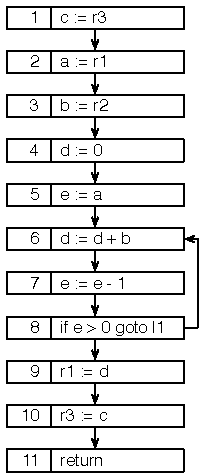
\includegraphics[scale=.85]{questions/register-allocation/controlflow-appel-11-3-1}}
  }
\begin{tabular}[t]{r|l>{\ttfamily}l>{\ttfamily}l|>{\ttfamily}l>{\ttfamily}l|>{\ttfamily}l>{\ttfamily}l}
node & succ & \textnormal{def} & \textnormal{use} & \textnormal{out} &
\textnormal{in} & \textnormal{out} & \textnormal{in} \\
\hline
11 &        &    &     & r1 r3   & r1 r3    & r1 r3   & r1 r3   \\
10 & 11     & r3 & c   & r1 r3   & r1 c     & r1 r3   & r1 c    \\
 9 & 10     & r1 & d   & r1 c    & c d      & r1 c    & c d     \\
 8 &  6, 9  &    & e   & c d     & c d e    & b c d e & b c d e \\
 7 &  8     & e  & e   & c d e   & c d e    & b c d e & b c d e \\
 6 &  7     & d  & b d & c d e   & b c d e  & b c d e & b c d e \\
 5 &  6     & e  & a   & b c d e & a b c d  & b c d e & a b c d \\
 4 &  5     & d  &     & a b c d & a b c    & a b c d & a b c   \\
 3 &  4     & b  & r2  & a b c   & r2 a c   & a b c   & r2 a c  \\
 2 &  3     & a  & r1  & r2 a c  & r1 r2 c  & r2 a c  & r1 r2 c \\
 1 &  2     & c  & r3  & r1 r2 c & r1 r2 r3 & r1 r2 c & r1 r2 r3
\end{tabular}
\end{solution}


\newpage             

\titledquestion{Register allocation}
\droptotalpoints

You have to colour the following interference graph with three colours
(\verb+r1+, \verb+r2+, \verb+r3+ are precoulored):
\vspace{-1em}
\begin{center}
  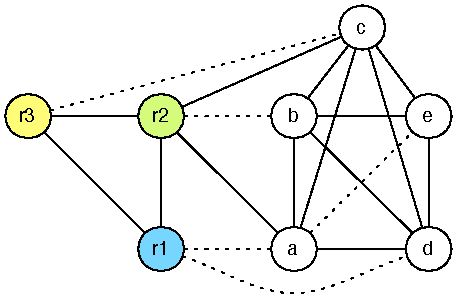
\includegraphics[scale=.85]{questions/register-allocation/interference-appel-11-3-1}
\end{center}

\begin{parts}
\part[5]
Should the next step be a \emph{spill}? Why (not)?

\begin{solution}
We cannot simplify, since all nodes are either precoloured or move-related.
But we can coalesce \Verb+a+ and \Verb+e+ (all neighbours of \Verb+e+
of significant degree are neighbors of \Verb+a+, George).
\end{solution}

\part[12]
Spill node \verb+c+ and continue the graph colouring until you can decide if this spill is an actual one.

\begin{solution}
We can coalesce \Verb+a+ and \Verb+e+, since the resulting node has no
neighbours of significant degree ($0<3$, Briggs).
For the same reason, we can coalesce \Verb+a e+ and \Verb+r1+ as well as
\Verb+b+ and \Verb+r3+.
We cannot coalesce \Verb+a e r1+ with \Verb+d+ since they interfere,
but we can simplify \Verb+d+.
Now we have only precoloured nodes and can bring back nodes, starting
with \Verb+d+.

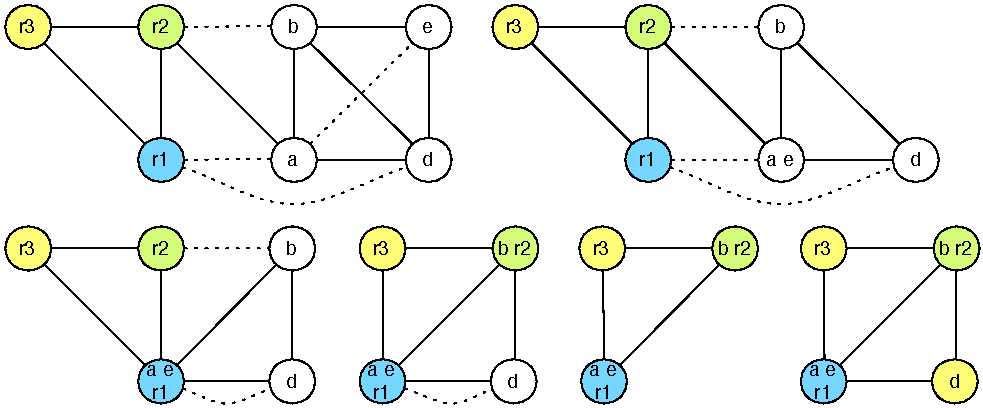
\includegraphics[scale=.85]{questions/register-allocation/colouring-appel-11-3-1}
\end{solution}

\part[1]
Is node \verb+c+ an actual spill?

\begin{solution}
Yes, since we cannot assign any colour to \Verb+c+.
\end{solution}

\part[2]
Perform the spill on the intermediate code from the previous question.

\begin{solution}
\begin{minipage}[t]{5cm}
\fvset{frame=lines}
\fvset{framesep=8pt}
\begin{Verbatim}
     c1 := r3
     M[cloc] := c1
     a := r1
     b := r2
     d := 0 
     e := a      
l1:  d := d + b
     e := e - 1
     if e > 0 goto l1
     r1 := d
     c2 := M[cloc]
     r3 := c2
     return     
\end{Verbatim}
\end{minipage}

\end{solution}

\end{parts}
 

\titledquestion{Garbage collection}
\droptotalpoints

\begin{parts}
\part[3]
Explain the general ideas behind garbage collection by reference counting.

\begin{solution}
For each element on the heap, a counter is maintained.
At each assignment, the counter of the olde reference is decreased
and the counter of the new reference increased.
Heap elements with a reference count of 0 can be collected when memory for
a new element needs to be allocated.
\end{solution}

\part[2]
What are the disadvantages of this strategy?

\begin{solution}
Heap elements with cyclic references are not collected.
Furthermore, the additional instructions for counting slow down the execution.
\end{solution}
\end{parts}

\titledquestion{Lexical analysis}
\droptotalpoints

Let $G_2$ be a formal grammar with nonterminal symbols $S$ and $D$,
terminal symbols '$\mathbf{b}$', '$\mathbf{0}$' and '$\mathbf{1}$', 
start symbol $S$, and the following production rules:
\begin{eqnarray*}
S & \rightarrow & \mathbf{b\ } D\\
D & \rightarrow & \mathbf{0\ } D\\
D & \rightarrow & \mathbf{1\ } D\\
D & \rightarrow & \mathbf{0}\\
D & \rightarrow & \mathbf{1}
\end{eqnarray*}

\begin{parts}

\part[1]
Is $G_2$ regular? Why (not)?

\begin{solution}
Yes.
All rules have only a single nonterminal symbol on their left-hand side and
either a single terminal symbol or a terminal symbol followed by a nonterminal
symbol on their right-hand side.
\end{solution}

\part[2]
Describe the language defined by $G_2$ in English.

\begin{solution}
The language consists of all words starting with \textbf{b}, followed by one or
more digits \textbf{0} or \textbf{1}, i.e. binary numbers marked with a leading
\textbf{b}.
\end{solution}

\part[4]
Turn $G_2$ \emph{systematically} into a finite automaton.

\begin{solution}
\vspace{-1em}
\begin{center}
  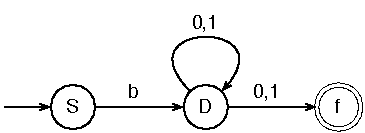
\includegraphics[scale=.85]{questions/lexical/binaries-nfa}
\end{center}
\end{solution}

\part[3]
Use $G_2$ to generate a word with at least five letters. 
Show each derivation step.
Use the automaton to recognise this word. 
Enumerate the states passed during the recognition.

\begin{solution}
\vspace{-1em}
\begin{displaymath}
S \Rightarrow 
\mathbf{b\ } D \Rightarrow 
\mathbf{b\ } \mathbf{1\ } D \Rightarrow 
\mathbf{b\ } \mathbf{1\ } \mathbf{0\ } D \Rightarrow 
\mathbf{b\ } \mathbf{1\ } \mathbf{0\ } \mathbf{1\ } D \Rightarrow 
\mathbf{b\ } \mathbf{1\ } \mathbf{0\ } \mathbf{1\ } \mathbf{0}
\end{displaymath}
\begin{displaymath}
S \stackrel{\mathbf{b}}{\rightarrow} 
D \stackrel{\mathbf{1}}{\rightarrow} 
D \stackrel{\mathbf{0}}{\rightarrow} 
D \stackrel{\mathbf{1}}{\rightarrow} 
D \stackrel{\mathbf{0}}{\rightarrow} 
f
\end{displaymath}

\end{solution}

\end{parts}

\titledquestion{LL parsing}
\droptotalpoints

Let $G_3$ be a formal grammar with nonterminal symbols $S$, $T$, $E$ and $E^\prime$,
terminal symbols '$\mathbf{x}$', '$\mathbf{+}$' and '$\mathbf{\$}$', start symbol $S$,
and the following production rules:
\begin{eqnarray*}
S & \rightarrow & E \mathbf{\ \$}\\
E & \rightarrow & T \  E^\prime \\
E^\prime & \rightarrow & \mathbf{+\ } \ T \  E^\prime \\
E^\prime & \rightarrow &  \\
T & \rightarrow & \mathbf{x} 
\end{eqnarray*}

\begin{parts}
\part[8]
Construct an LL(0) parse table for the grammar. 
Calculate FIRST and FOLLOW sets as needed.

\begin{solution}
\begin{tabular}[t]{l|lll}
     & nullable & FIRST & FOLLOW \\
\hline
$S$ & no & $\mathbf{x}$ & \\
$E$ & no & $\mathbf{x}$ & $\mathbf{\$}$ \\
$E^\prime$ & yes & $\mathbf{+}$ & $\mathbf{\$}$ \\
$T$ & no & $\mathbf{x}$ & $\mathbf{+}\,\mathbf{\$}$
\end{tabular}
\begin{tabular}[t]{l|ccc}
     & $\mathbf{x}$ & $\mathbf{+}$ & $\mathbf{\$}$ \\
\hline
$S$ & $S \rightarrow E \mathbf{\ \$}$\\
$E$ & $E \rightarrow T \  E^\prime$\\
$E^\prime$ & & $E^\prime \rightarrow \mathbf{+\ } \ T \  E^\prime$ & $E^\prime
\rightarrow$\\
$T$ & $T \rightarrow \mathbf{x}$
\end{tabular}
\end{solution}

\part[2]
Use the parse table to recognise the sentence $\mathbf{x+x}$.
Show the stack and the remaining input after each step.

\begin{solution}
\begin{tabular}[t]{r|r}
stack & input \\
\hline
$S$   & $\mathbf{x+x\$}$ \\
$E\$$ & $\mathbf{x+x\$}$ \\
$TE^\prime\$$ & $\mathbf{x+x\$}$ \\
$\mathbf{x}E^\prime\$$ & $\mathbf{x+x\$}$ \\
% \end{tabular}
% \begin{tabular}[t]{r|r}
% stack & input \\
% \hline
$E^\prime\$$ & $\mathbf{+x\$}$ \\
$\mathbf{+} T E^\prime\$$ & $\mathbf{+x\$}$ \\
$T E^\prime\$$ & $\mathbf{x\$}$ \\
$\mathbf{x} E^\prime\$$ & $\mathbf{x\$}$ \\
% \end{tabular}
% \begin{tabular}[t]{r|r}
% stack & input \\
% \hline
$E^\prime\$$ & $\mathbf{\$}$ \\
$\mathbf{\$}$ & $\mathbf{\$}$
\end{tabular}
\end{solution}

\end{parts}


\end{questions}

\end{document}
